\graphicspath{{chapters/chapter4/}}
\chapter{Research Method}

\section{Solution Construction}

\subsection{Introduction}
The minimum cost flow problem can intuitively be represented as a graph problem where the goal is to find the cheapest way to flow a commodity through your graph. This section discusses three solution construction methods that were proposed to generate ant solution to the MCFP domain.

\subsection{Alternated Move and Push}\label{sec:alternated_move_and_push}

This first approach is also the most naturalistic solution construction method that was considered. The idea was to repeatedly let an ant walk along a path from the source to a sink node until the ant trails formed a network that connected all demand nodes to the source node. Empirically, this approach was strongly rooted in nature, where ant colonies have to organize trail systems leading to food sources in their environment.

This strategy entails an incremental solution construction, where a single solution is constructed by letting the ant walk through the graph multiple times. An illustration of the procedure is depicted in \Cref{fig:alternated_move_and_push_construction}. At each junction the ant faces, it chooses one of the paths randomly. Expressed in a different way, the solution is constructed by a series of local decisions and can be characterized as a decentralized strategy.

\begin{figure}[htp] % (here, top of the page, the next page)
\graphicspath{{chapters/chapter4/images/alternated_move_and_push/}}
%\centering

\begin{subfigure}[t]{0.30\textwidth}
  \centering
  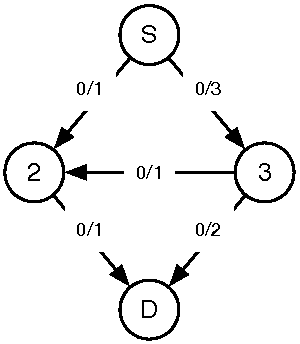
\includegraphics[width=\linewidth,height=\linewidth, keepaspectratio]{alternated_move_and_push1.pdf}
  \caption{A capacitated graph with one source $S$ and one sink $D$ node.}\label{fig:alternated_move_and_push_fig1}
\end{subfigure}
\quad
\begin{subfigure}[t]{0.30\textwidth}
  \centering
  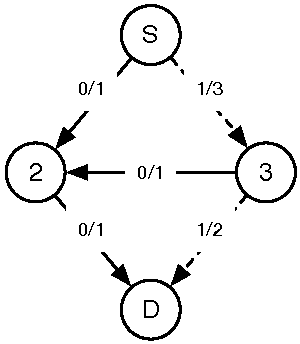
\includegraphics[width=\linewidth,height=\linewidth, keepaspectratio]{alternated_move_and_push2.pdf}
  \caption{The first trail created by an ant. The path is randomly created based on pheromone levels. A single flow unit is pushed along the the edges included in the trail. The trail is denoted by a dashed line.}\label{fig:alternated_move_and_push_fig2}
\end{subfigure}
\quad
\begin{subfigure}[t]{0.30\textwidth}
  \centering
  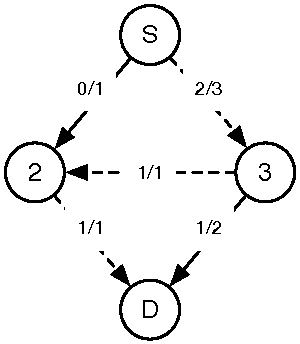
\includegraphics[width=\linewidth,height=\linewidth, keepaspectratio]{alternated_move_and_push3.pdf}
  \caption{A second pass is conducted by the same ant. This resulted in a new random path. A single flow unit is pushed along the trail.}\label{fig:alternated_move_and_push_fig3}
\end{subfigure}

\begin{subfigure}[t]{0.30\textwidth}
  \centering
  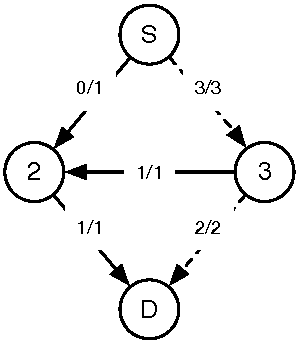
\includegraphics[width=\linewidth,height=\linewidth, keepaspectratio]{alternated_move_and_push4.pdf}
  \caption{A third pass is performed by the same ant, and a flow unit is pushed through the graph along the path.}\label{fig:alternated_move_and_push_fig4}
\end{subfigure}
\quad
\begin{subfigure}[t]{0.30\textwidth}
  \centering
  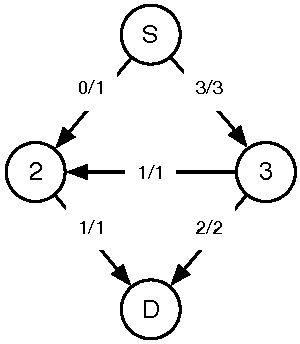
\includegraphics[width=\linewidth,height=\linewidth, keepaspectratio]{alternated_move_and_push5.pdf}
  \caption{The ant can no longer reach the sink node, and the ant therefore terminates its search for paths through the graph. The solution construction has terminated.}\label{fig:alternated_move_and_push_fig5}
\end{subfigure}


\caption{How a solution is constructed using the Alternated Move and Push strategy.}\label{fig:alternated_move_and_push_construction}
\end{figure}

The Alternated Move and Push strategy is proof that a system of simple agents are able to cooperate through interaction with the environment and solve flow path problems. This procedure is a general solver for capacitated edge problems. If the problem can be described as a graph with edges, the ants can be used as a meta-solver. Whether the problem is to find the maximum flow and minimum cost, or to find the shortest TSP; the ants are dependant upon the edges pheromone level. This abstraction of the problem domain enables the strategy to be used as a general solver.

\subsubsection{Application to the MCFP domain}
In order to apply this approach to solve problems in the MCFP domain we have to transform the problem into a capacitated graph. This was easily achieved through a three step process. First, we add a super-sink to the graph. The super-sink will be the only demand node. Second, we add edges leading for each demand node into the super-sink. Finally, we infinite capacity to the internal edges, while the edges leading to the super-sink has a capacity equal to the demand of the originating node. 

\begin{figure}[htb]
   \center 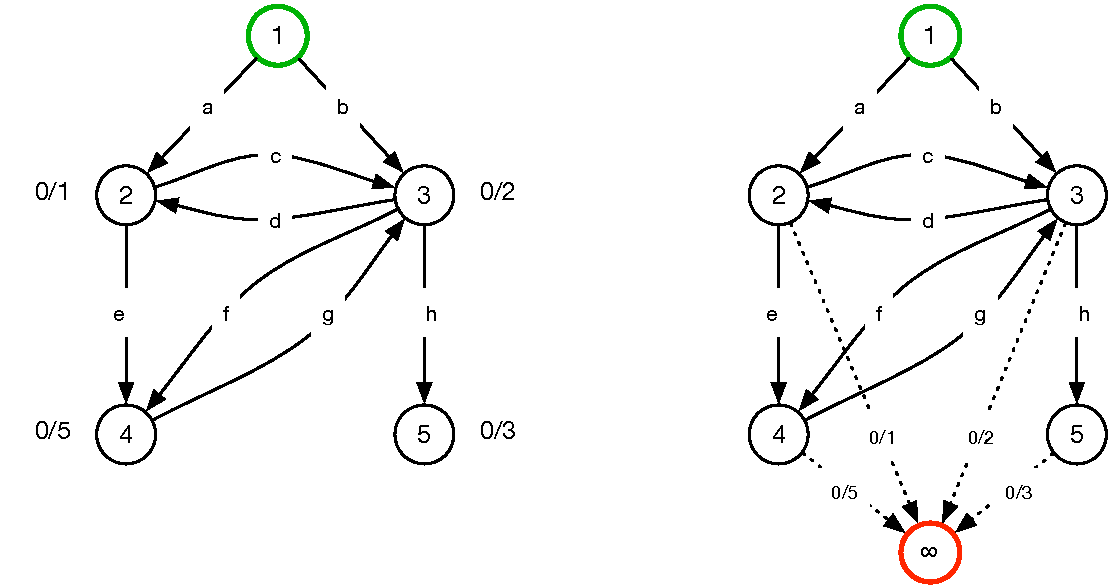
\includegraphics[width=0.8\linewidth,height=0.4\linewidth, keepaspectratio]{images/introduce_supersink.pdf}
   \caption[Introducting a super-sink to MCFP]{Introducing a super-sink to the uncapacitated single source, multiple sink minimum cost flow problem.}\label{fig:MCFP-supersink}
\end{figure}

The result of this process is depicted in \Cref{fig:MCFP-supersink}. The demand from demand nodes $D = {2, 3, 4, 5}$ has been replaced by capacitated edges into the supersink. The capacity of the corresponding edge mirror the demand of the starting node.


\subsection{Depth First Search}
Construct a tree using a stochastic depth first search where the edges are chosen proportionately to their pheromone.

When surveying \Cref{fig:alternated_move_and_push_construction} and analyzing the solution construction approach in \fullref{sec:alternated_move_and_push}, we can deduct that the solutions produced by a single ant shares similarities with a depth first search. The ant is consecutively faced with edge conjunctions in the graph until it reaches the supersink.

\subsection{Spanning Tree Construction}
Construct stochastic MSTs of the graph where the edges are chosen proportionately to their pheromone. All min cost solution will be trees.

Hvis vi definerer et MST som den korteste veien fra en root node til alle andre noder. Hvis vi så tenker at vi lar kosten det tar å flyte en commodity langs en kant tilsvare avstanden mellom to noder, kan vi tenke at å konstruere en MST fra source-noden vår vil produsere nærmere optimale løsninger. Konstruere en MST fra root noden er det samme NP komplette problemet som å løse MCFP. Hvordan kan vi ameliorate dette? Vi kan ikke være grådige og må heller bruke en randomisert approach. La oss heller konstruere MSTet hvor sannsynligheten for å inkludere en gitt edge er proposjonal med som pheromonverdien til den gitte kanten. Vi vet at når $t \rightarrow \infty$, vil kantene som er med i den beste løsningen ha mye mer pheromoner andre kanter. Dermed vil vi i limit ha mye større sannsynglihet for å generere det optimale MST.

\subsection{Example: Constructing a Solution}
Show how a solution (for a simple problem) is constructed.

%
% End Solution Construction


\section{ACO Self-Reinforcement Algorithm}
En god beskrivelse av algoritmen. Vis hvordan reinformencent fungerer. Hvordan den velger nye løsninger å følge. Vis hvordan algoritmen bruker en prioritetsliste. Vis hvorfor dette kan unngå stagnation. Spar analysen til analysekapittelet.
\paragraph{Show} how a typical run would look in terms of discovering the solution and avoiding stagnation.

%
% End ACO Self-Reinforcement Algorithm


\section{ACO Threshold-Information Algorithm}
Forklar hvordan vi bruker stagnering som en stimuli for å oppføre seg som scouts. Forklar hvordan thresholding er brukt til å bytte oppgaver. Forklar intuisjonen for hvorfor dette vil hindre stagnering. Vis hvordan scoutene vil prøve å finne nye gode løsninger rundt den globale løsningen. 

\begin{itemize}
    \item[] \textbf{show} how a typical run would look in terms of discovering the solution and avoiding stagnation.
    \item[] \textbf{local decisions} explain how this is a decentralized solver. Selecting edges at each intersection.
    \item[] \textbf{not a random restart} guided towards the global solution. (show a graph)
\end{itemize}

%
% End ACO Threshold-Information Algorithm


\section{Experiment}
Describe some of the graphs and list our assumptions.

\subsection{Parameter Settings}
\begin{itemize}
    \item[] \textbf{how did we find them?} exhaustive search on a large graph set
    \item[] \textbf{optimal parameter} list the configuration
\end{itemize}